\documentclass[border=10pt]{standalone}

\usepackage{tikz}
\usepackage{tikzsymbols}
\usetikzlibrary{calc,patterns,shapes.geometric}

\def\centerarc[#1](#2)(#3:#4:#5){\draw[#1] ($(#2)+({#5*cos(#3)},{#5*sin(#3)})$) arc (#3:#4:#5);}

\begin{document}
	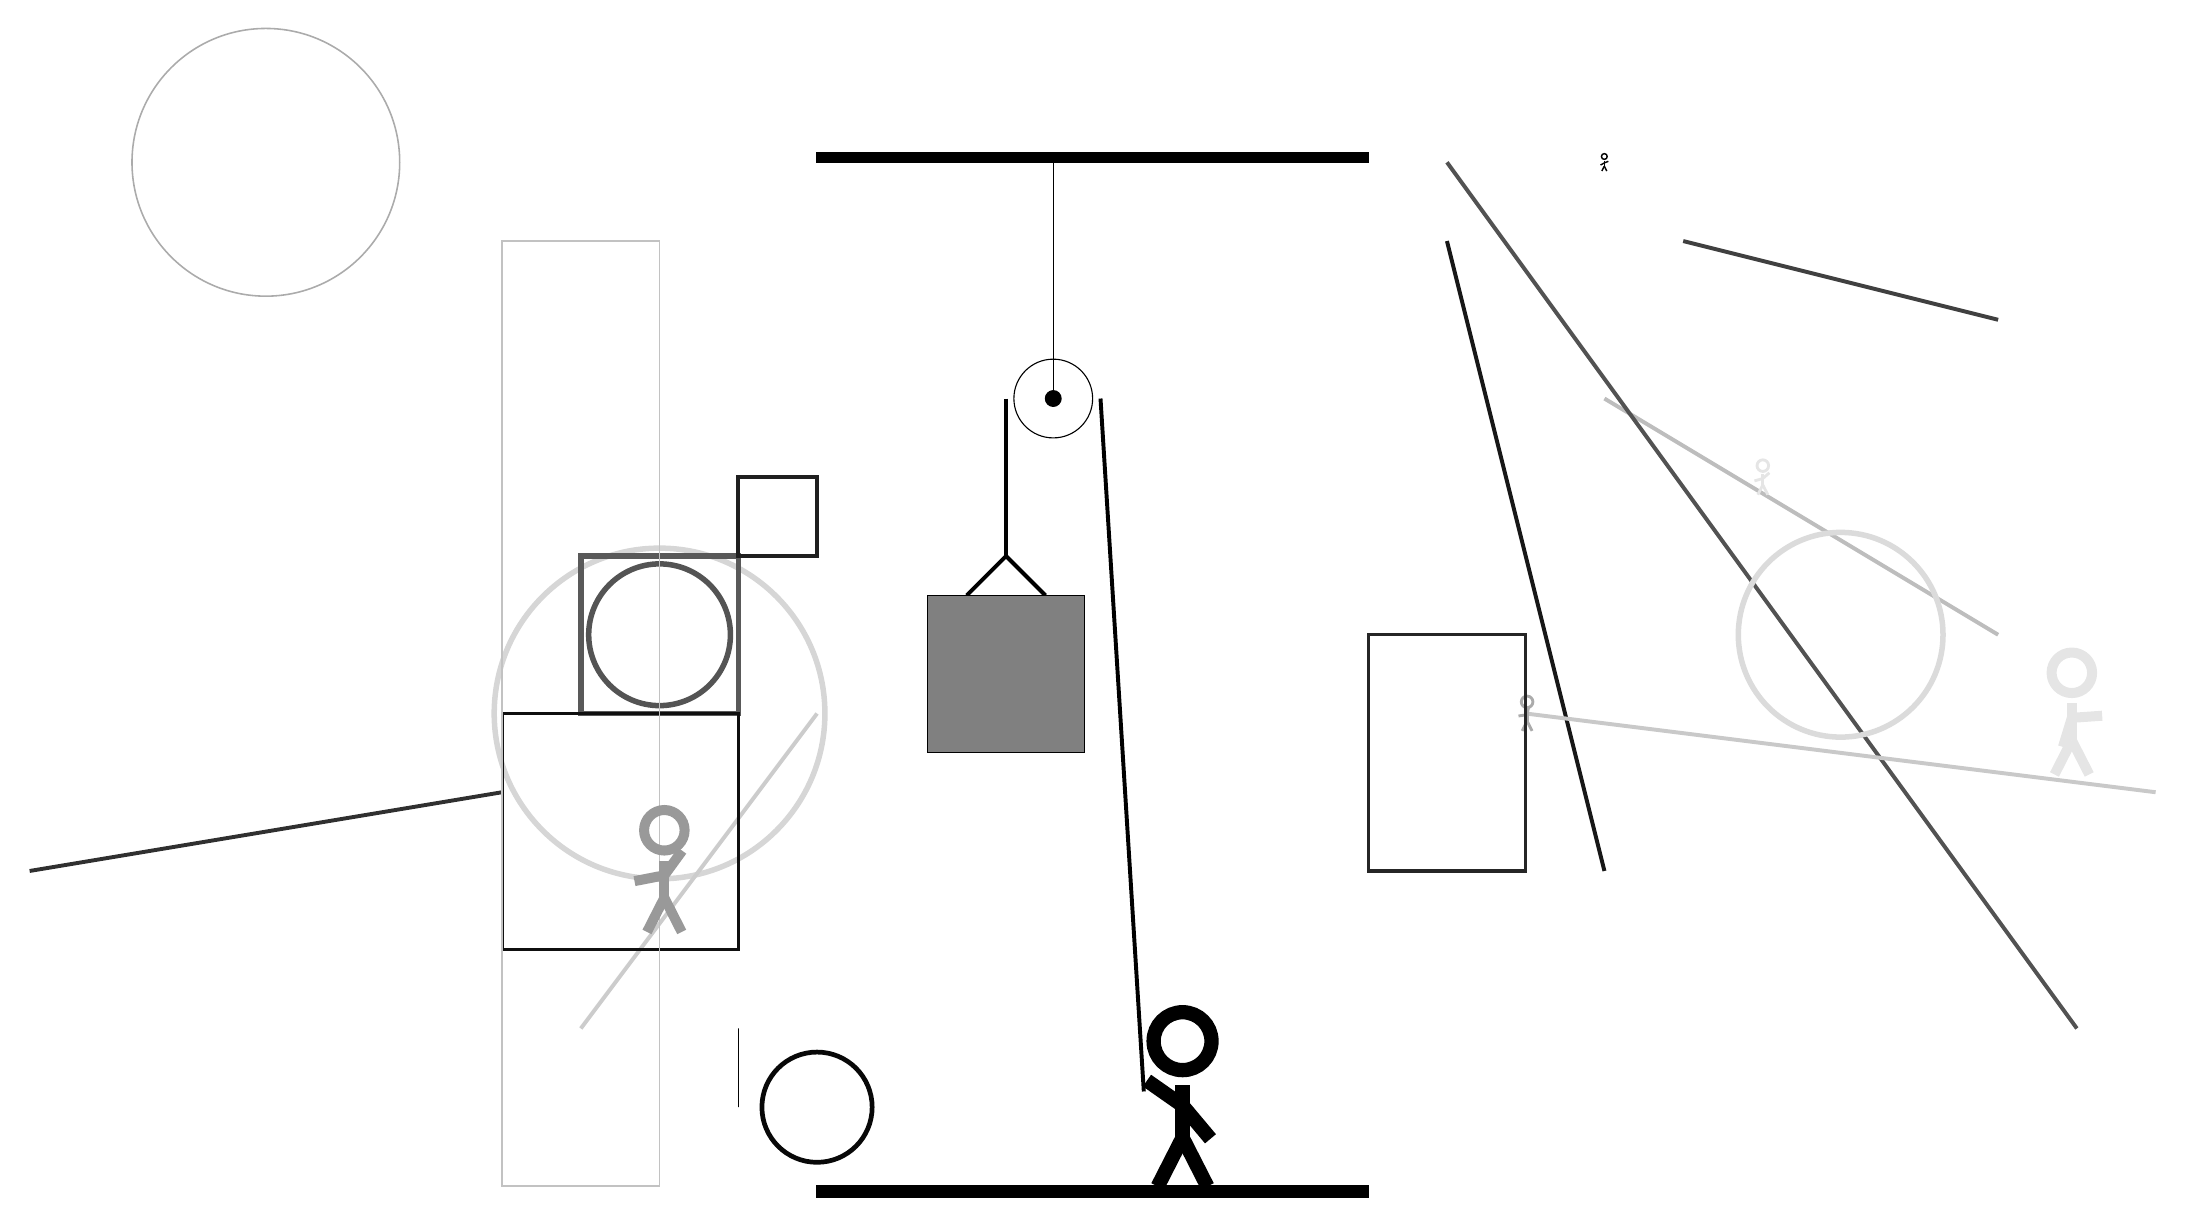
\begin{tikzpicture}
		%%%%% START %%%%%
		
		\draw[fill=black] (-2, 10) rectangle (5, 10.125);
		
		\draw (1, 7) circle (0.5);
		\draw[fill=black] (1, 7) circle (0.1);
		\draw (1, 10) -- (1, 7);
		
		\draw[line width=0.5mm] (-0.1, 4.5) -- (0.4, 5.0) -- (0.9, 4.5);
		\draw[fill=black!50] (-0.6, 4.5) rectangle (1.4, 2.5);
		
		\draw[line width=0.5mm] (0.4, 7) -- (0.4, 5.0);
		\centerarc[line width=0.5mm](1, 7)(0:180:0.6);
		\draw[line width=0.5mm](1.6, 7) -- (2.15, -1.8);
		
		\node at (2.6, -1.9) {\Strichmaxerl[10][-35][-50]};
		
		\draw[line width=0.5mm, color=black!91](6, 9) -- (8, 1);
		
		\draw[line width=0.5mm, color=black!26](8, 7) -- (13, 4);
		\draw[line width=0.5mm, color=black!68](6, 10) -- (14, -1);
		\draw[line width=0.5mm, color=black!21](7, 3) -- (15, 2);
		
		\node[line width=0.4mm, color=black!33] at (7, 3) {\Strichmaxerl[2][8][79]};
		\draw [line width=0.7mm, color=black!16](-4, 3) circle (2.1);
		\node[line width=0.5mm, color=black!10] at (10, 6) {\Strichmaxerl[2][16][41]};
		
		\draw[line width=0.5mm, color=black!20](-2, 3) -- (-5, -1);
		\draw[line width=0.5mm, color=black!81](-6, 2) -- (-12, 1);
		\draw[line width=0.7mm, color=black!65] (-3, 3) rectangle (-5, 5);
		\draw[line width=0.2mm, color=black!99] (-3, -2) rectangle (-3, -1);
		
		\draw [line width=0.7mm, color=black!67](-4, 4) circle (0.9);
		\draw[line width=0.4mm, color=black!94] (-3, 0) rectangle (-6, 3);
		
		\node[line width=0.3mm, color=black!99] at (8, 10) {\Strichmaxerl[1][29][22]};
		\draw[line width=0.5mm, color=black!75](9, 9) -- (13, 8);
		\draw[line width=0.2mm, color=black!24] (-4, 9) rectangle (-6, -3);
		\draw [line width=0.6mm, color=black!97](-2, -2) circle (0.7);
		\draw[line width=0.4mm, color=black!85] (5, 4) rectangle (7, 1);
		\node[line width=0.4mm, color=black!40] at (-4, 1) {\Strichmaxerl[7][11][54]};
		
		\draw [line width=0.7mm, color=black!14](11, 4) circle (1.3);
		\draw[line width=0.5mm, color=black!88] (-2, 6) rectangle (-3, 5);
		
		\node[line width=0.6mm, color=black!10] at (14, 3) {\Strichmaxerl[7][73][4]};
		\draw [line width=0.2mm, color=black!33](-9, 10) circle (1.7);
		
		\draw[fill=black] (-2, -3) rectangle (5, -3.15);
		
		%%%%% END %%%%%
	\end{tikzpicture}
\end{document}